\section{Arquitecturas}
Esta sección describe la arquitectura de alto nivel del sistema \textbf{QuickContentMedia}, definiendo cómo se organizan e interconectan sus principales componentes. Se presentan tanto la estructura lógica del software (mediante el diagrama de componentes), como su distribución física en el entorno de ejecución (mediante el diagrama de despliegue).

\subsection{Componentes}

La figura \ref{DiagComp} muestra el diagrama de componentes que modela la estructura lógica del sistema \textbf{QuickContentMedia}, mostrando los componentes principales y las interfaces para su interacción.

\begin{figure}[H]
    \centering
    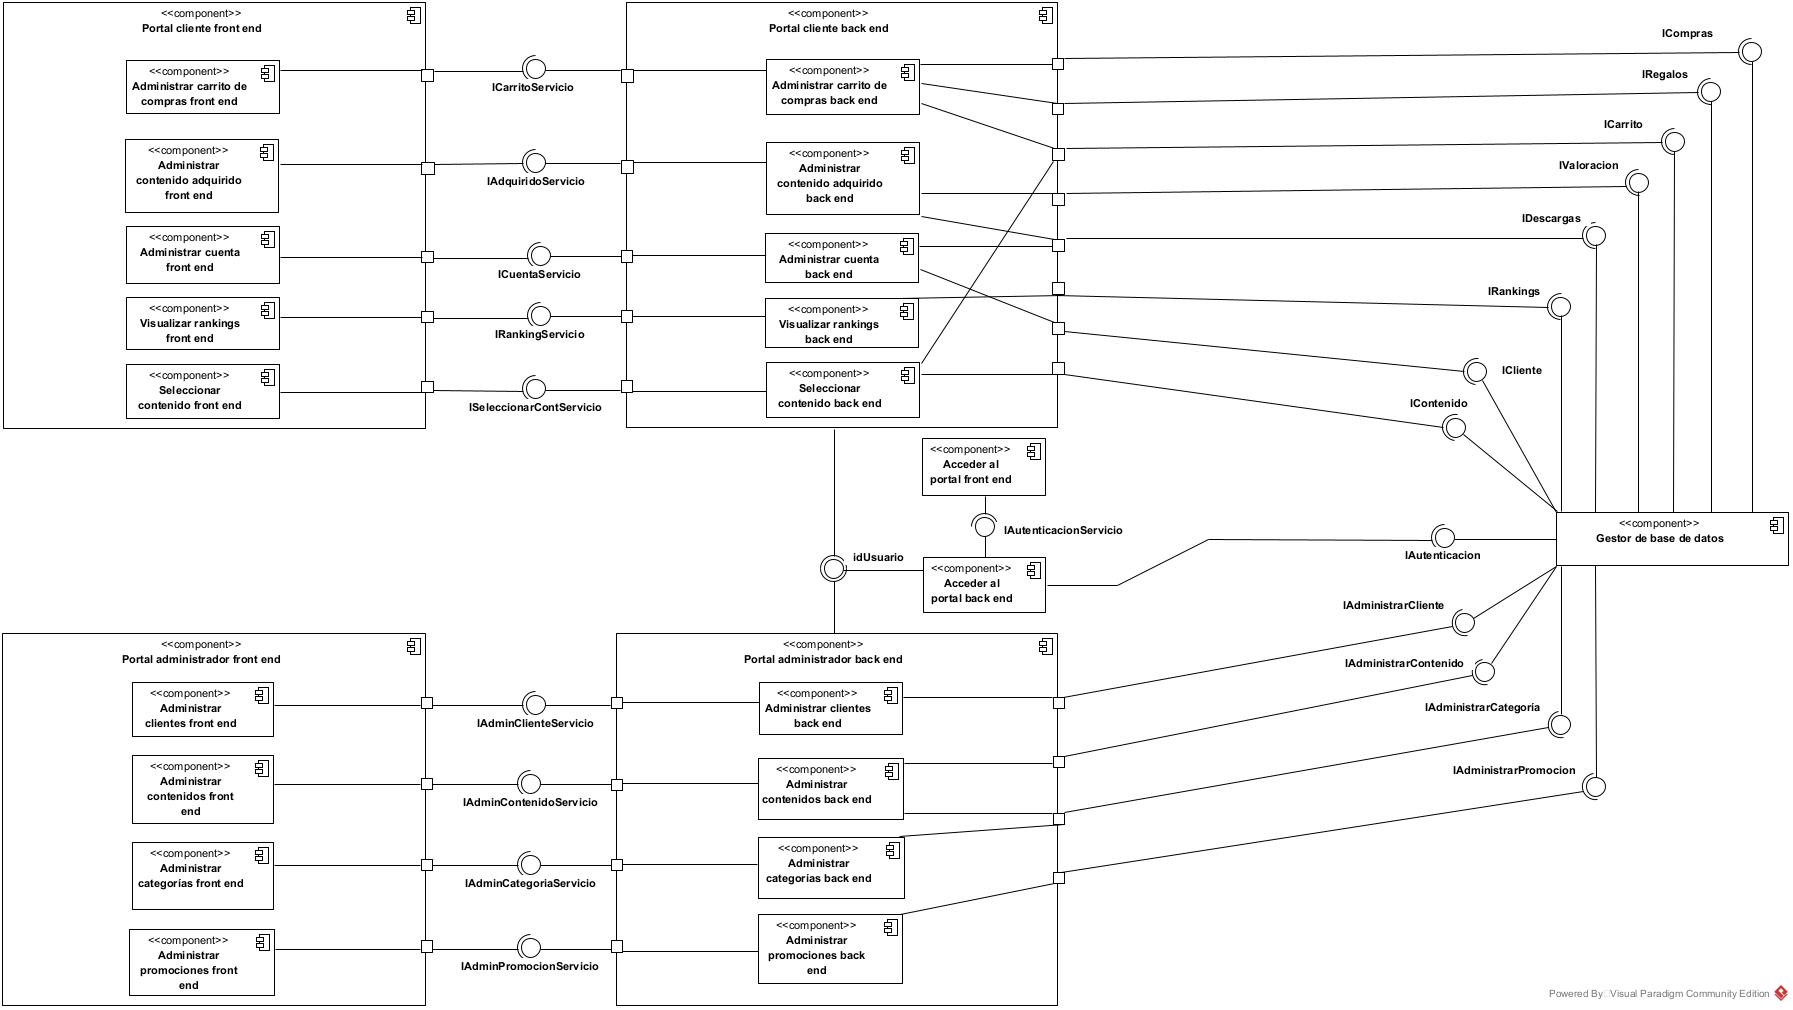
\includegraphics[width=0.95\linewidth]{Media/4_Disenio/componentes.jpg}
    \caption{Diagrama de componentes del sistema \textbf{QuickContentMedia}}
    \label{DiagComp}
\end{figure}

\textbf{Archivo:} Diagrama de componentes (formato Visual Paradigm) \\
\textbf{Link de descarga:} \linkDiagramaComponentes \\

\textbf{Pasos de ejecución:}
\begin{itemize}
    \item Ingresar al repositorio en GitHub usando el link proporcionado y descargar el archivo \texttt{QCM.vpp}.
    \item En la pestaña Component Diagram abrir DiagramaComponentesQCM.
\end{itemize}

\subsubsection{Diccionario de componentes}

%Parte1

\begin{longtable}{|p{3.3cm}|p{1.2cm}|p{5cm}|p{2.0cm}|p{3.5cm}|}
\caption{Diccionario de componentes (Parte 1)}
\label{tab:diccionario_componentes_1} \\

\hline
\textbf{Nombre} & \textbf{ID} & \textbf{Descripción} & \textbf{Requisitos implementados} & \textbf{Clases} \\ \hline
\endfirsthead

\hline
\textbf{Nombre} & \textbf{ID} & \textbf{Descripción} & \textbf{Requisitos implementados} & \textbf{Clases} \\ \hline
\endhead

Administrar carrito de compras front end & CT-001 & Vista para gestionar el carrito desde el cliente & RF-005 & UICarrito\newline UIDestinatario\newline UIResumenPedido \\ \hline
Administrar contenido adquirido front end & CT-002 & Vista que muestra el contenido comprado por el usuario & RF-006 &UIMisContenidos \\ \hline
Administrar cuenta front end & CT-003 & Vista para que el usuario gestione su cuenta personal & RF-003\newline RF-004 &UIPerfilCliente\newline UIOpcionesRecarga \\ \hline
Visualizar rankings front end & CT-004 & Vista que muestra los rankings de contenido más popular & RF-007 &UIRankingDescarga\newline UIRankingValoracion\newline UIRankingClientes \\ \hline
Seleccionar contenido front end & CT-005 & Vista para navegar y seleccionar contenido para compra & RF-002 &UIInicioCliente\newline UIVideoImagen\newline UISonido \\ \hline
Administrar carrito de compras back end & CT-006 & Lógica para procesar operaciones del carrito en el servidor & RF-005 & gestorCarrito \\ \hline
Administrar contenido adquirido back end & CT-007 & Lógica para gestionar datos del contenido adquirido & RF-006 & gestorCompra \\ \hline
Administrar cuenta back end & CT-008 & Lógica para manejar la información de la cuenta del usuario & RF-003\newline RF-004 &gestorUsuario \\ \hline
Visualizar rankings back end & CT-009 & Lógica para proporcionar datos de rankings de clientes y contenidos & RF-007 & gestorRanking \\ \hline
Seleccionar contenido back end & CT-010 & Lógica para gestionar la selección de contenido & RF-002 & gestorContenido\\ \hline


\end{longtable}

% Parte 2

\begin{longtable}{|p{3.3cm}|p{1.2cm}|p{5cm}|p{2.0cm}|p{3.5cm}|}
\caption{Diccionario de componentes (Parte 2)}
\label{tab:diccionario_componentes_2} \\

\hline
\textbf{Nombre} & \textbf{ID} & \textbf{Descripción} & \textbf{Requisitos implementados} & \textbf{Clases} \\ \hline
\endfirsthead

\hline
\textbf{Nombre} & \textbf{ID} & \textbf{Descripción} & \textbf{Requisitos implementados} & \textbf{Clases} \\ \hline
\endhead
Administrar clientes front end & CT-011 & Vista para administrar usuarios desde el cliente & RF-008 &UIAdministrarCliente \\ \hline
Administrar contenidos front end & CT-012 & Vista para administrar contenidos disponibles & RF-010 &UIAdministrarContenido \\ \hline
Administrar categorías front end & CT-013 & Vista para gestionar las categorías del sistema & RF-011 &UIAdministrarCategoria \\ \hline
Administrar promociones front end & CT-014 & Vista para gestionar promociones y descuentos & RF-009 &UIAdministrarPromoccion \\ \hline
Administrar clientes back end & CT-015 & Lógica para administrar los usuarios del sistema & RF-008 & gestorUsuario \\ \hline
Administrar contenidos back end & CT-016 & Lógica para gestionar los contenidos del sistema & RF-010 & gestorContenido \\ \hline
Administrar categorías back end & CT-017 & Lógica para administrar las categorías del sistema & RF-011 & gestorCategoria \\ \hline
Administrar promociones back end & CT-018 & Lógica para gestionar promociones y descuentos & RF-009 &gestorPromocion \\ \hline
Acceder al portal front end & CT-019 & Vista de inicio de sesión para usuarios y administradores & RF-001 &UIAccesoAlPortal\newline UIRegistroCliente \\ \hline
Acceder al portal back end & CT-020 & Lógica para verificar credenciales y redirigir al portal correspondiente & RF-001 &gestorUsuario \\ \hline
Gestor de base de datos & CT-021 & Lógica para el almacenamiento y recuperación de datos persistentes &RNF-001 & Clientes\newline Administradores\newline Carrito\_compras\newline Compras\newline Promociones\newline Contenidos\newline Categorías\newline Ranking\\ \hline

\end{longtable}
\newpage
\subsubsection{Diccionario de interfaces}

%PARTE 1
\begin{longtable}{|p{5cm}|p{4cm}|p{3.5cm}|p{3.5cm}|}
\caption{Diccionario de interfaces (Parte 1)}
\label{tab:diccionario_interfaces_1} \\

\hline
\textbf{Interfaz} & \textbf{Operaciones} & \textbf{Recibe} & \textbf{Devuelve} \\ \hline
\endfirsthead

\hline
\textbf{Interfaz} & \textbf{Operaciones} & \textbf{Recibe} & \textbf{Devuelve} \\ \hline
\endhead

\multirow{4}{5cm}{ICarritoServicio} 
    & obtenerContenidoCarrito & ID de usuario & Lista de ítems del carrito \\ \cline{2-4}
    & aplicarDescuentos & ID del usuario y su carrito & void \\ \cline{2-4}
    & eliminarContenido & ID del usuario y del contenido & Resultado de eliminación \\ \cline{2-4}
    & verificarDestinatario & ID de usuario destinatario & Resultado de validación \\ \hline
\multirow{3}{5cm}{IAdquiridoServicio} 
    & obtenerContenidosAdquiridos & ID del cliente & Lista de contenidos adquiridos \\ \cline{2-4}
    & registrarCalificacion & ID del cliente, ID del contenido, puntaje & void \\ \cline{2-4}
    & obtenerArchivo & ID del contenido & Archivo descargable \\ \hline
\multirow{4}{5cm}{ICuentaServicio} 
    & obtenerUsuario & ID del cliente & Datos del cliente \\ \cline{2-4}
    & validarContraseña & Contraseña actual y nueva & Booleano \\ \cline{2-4}
    & verificarSaldo & ID del cliente & Saldo disponible \\ \cline{2-4}
    & obtenerContenidos & ID del cliente & Contenidos descargados \\ \hline
\multirow{3}{5cm}{IRankingServicio} 
    & obtenerRankingDescarga & Ninguno & Lista de ranking de descargas \\ \cline{2-4}
    & obtenerRankingValoracion & Ninguno & Lista de ranking de valoraciones \\ \cline{2-4}
    & obtenerRankingClientes & Ninguno & Lista de ranking de clientes \\ \hline
\multirow{4}{5cm}{ISeleccionarContServicio} 
    & obtenerContenidos & Ninguno & Lista de contenidos \\ \cline{2-4}
    & obtenerContenidosPromocion & ID de promoción & Lista de contenidos en promoción \\ \cline{2-4}
    & obtenerContenidoPorAutor & Nombre del autor & Lista de contenidos del autor \\ \cline{2-4}
    & obtenerContenidoPorCategoria & Nombre de la categoría & Lista de contenidos de la categoría \\ \hline
\multirow{2}{5cm}{IAutenticacionServicio} 
    & validarCredenciales & Username y contraseña & Booleano \\ \cline{2-4}
    & registrarCredenciales & Username, contraseña, apellido, nombre & Booleano \\ \hline

\end{longtable}

%PARTE 2
\begin{longtable}{|p{5cm}|p{4cm}|p{3.5cm}|p{3.5cm}|}
\caption{Diccionario de interfaces (Parte 2)}
\label{tab:diccionario_interfaces_2} \\

\hline
\textbf{Interfaz} & \textbf{Operaciones} & \textbf{Recibe} & \textbf{Devuelve} \\ \hline
\endfirsthead

\hline
\textbf{Interfaz} & \textbf{Operaciones} & \textbf{Recibe} & \textbf{Devuelve} \\ \hline
\endhead

\multirow{3}{5cm}{IAdminClienteServicio} 
    & obtenerClientes & Ninguno & Lista de clientes \\ \cline{2-4}
    & obtenerContenidosDescargados & ID del cliente & Lista de contenidos descargados \\ \cline{2-4}
    & asignarSaldo & ID del cliente, monto de saldo & void \\ \hline
\multirow{5}{5cm}{IAdminContenidoServicio} 
    & obtenerContenidos & Ninguno & Lista de contenidos \\ \cline{2-4}
    & obtenerCategorias & Ninguno & Lista de categorías \\ \cline{2-4}
    & agregarContenido & Objeto contenido & void \\ \cline{2-4}
    & editarContenido & Objeto contenido & void \\ \cline{2-4}
    & eliminarContenido & ID del contenido & void \\ \hline
\multirow{3}{5cm}{IAdminCategoriaServicio} 
    & obtenerCategorias & Ninguno & Lista de categorías \\ \cline{2-4}
    & validarCategoria & Nombre y ruta de la categoría & Booleano \\ \cline{2-4}
    & renombrarCategoria & ID y nuevo nombre de la categoría & void \\ \hline
\multirow{6}{5cm}{IAdminPromocionServicio} 
    & obtenerPromociones & Ninguno & Lista de promociones \\ \cline{2-4}
    & obtenerContenidoPromocion & ID de promoción & Lista de contenidos en promoción \\ \cline{2-4}
    & verificarPromocion & ID del contenido & Lista de promociones relacionadas \\ \cline{2-4}
    & registrarPromocion & Objeto promoción & void \\ \cline{2-4}
    & actualizarPromocion & Objeto promoción actualizado & void \\ \cline{2-4}
    & eliminarPromocion & ID de la promoción & void \\ \hline
\multirow{1}{5cm}{ICompras} 
    & guardarCompra & ID del cliente, ID del contenido & void \\ \hline
\multirow{1}{5cm}{IRegalos} 
    & guardarRegalo & ID del cliente emisor, ID del cliente destinatario, ID del contenido & void \\ \hline
\multirow{4}{5cm}{ICarrito}
    & obtenerContenidosCarrito & ID del cliente & Lista de contenidos \\ \cline{2-4}
    & actualizarCampoDescuento & ID del cliente, ID del contenido & Booleano \\ \cline{2-4}
    & eliminarContenido & ID del cliente, ID del contenido & Booleano \\ \cline{2-4}
    & eliminarTodo & ID del cliente & void \\ \hline

\end{longtable}

%PARTE 3
\begin{longtable}{|p{5cm}|p{4cm}|p{3.5cm}|p{3.5cm}|}
\caption{Diccionario de interfaces (Parte 3)}
\label{tab:diccionario_interfaces_3} \\

\hline
\textbf{Interfaz} & \textbf{Operaciones} & \textbf{Recibe} & \textbf{Devuelve} \\ \hline
\endfirsthead

\hline
\textbf{Interfaz} & \textbf{Operaciones} & \textbf{Recibe} & \textbf{Devuelve} \\ \hline
\endhead

\multirow{1}{5cm}{IValoracion} 
    & agregarValoracion & ID del cliente, ID del contenido, puntaje & void \\ \hline
\multirow{1}{5cm}{IDescargas} 
    & obtenerContenidosDescargados & ID del cliente & Lista de contenidos descargados \\ \hline
\multirow{3}{5cm}{IRankings} 
    & obtenerRankingDescarga & Ninguno & Datos del ranking de descargas \\ \cline{2-4}
    & obtenerRankingValoracion & Ninguno & Datos del ranking de valoraciones \\ \cline{2-4}
    & obtenerRankingClientes & Ninguno & Datos del ranking de clientes \\ \hline
\multirow{3}{5cm}{ICliente} 
    & obtenerUsuario & ID del cliente & Datos del cliente \\ \cline{2-4}
    & validarContraseña & Contraseña actual y nueva & Booleano \\ \cline{2-4}
    & verificarSaldo & ID del cliente & Saldo disponible \\ \hline
\multirow{4}{5cm}{IContenido} 
    & obtenerContenidos & Ninguno & Lista de contenidos \\ \cline{2-4}
    & agregarContenido & Objeto contenido & void \\ \cline{2-4}
    & editarContenido & Objeto contenido & void \\ \cline{2-4}
    & eliminarContenido & ID del contenido & void \\ \hline
\multirow{3}{5cm}{IAutenticacion} 
    & validarCredenciales & Username, contraseña & Booleano \\ \cline{2-4}
    & validarUsername & Username & Booleano \\ \cline{2-4}
    & registrarCredenciales & Username, apellido, contraseña, nombre & void \\ \hline
\multirow{2}{5cm}{IAdministrarCliente} 
    & obtenerClientes & Ninguno & Lista de clientes \\ \cline{2-4}
    & asignarSaldo & ID del cliente, monto de saldo & void \\ \hline
\multirow{3}{5cm}{IAdministrarContenido} 
    & agregarContenido & Objeto contenido & void \\ \cline{2-4}
    & editarContenido & Objeto contenido & void \\ \cline{2-4}
    & eliminarContenido & ID del contenido & void \\ \hline
\multirow{2}{5cm}{IAdministrarCategoria} 
    & validarCategoria & Nombre y ruta de la categoría & Booleano \\ \cline{2-4}
    & renombrarCategoria & ID de la categoría, nuevo nombre & void \\ \hline
\multirow{4}{5cm}{IAdministrarPromocion} 
    & verificarPromocion & ID del contenido & Lista de promociones relacionadas \\ \cline{2-4}
    & registrarPromocion & Objeto promoción & void \\ \cline{2-4}
    & actualizarPromocion & Objeto promoción & void \\ \cline{2-4}
    & eliminarPromocion & Objeto promoción & void \\ \hline

\end{longtable}

\newpage
\subsection{Despliegue}

La figura \ref{DiagDesp} representa cómo se despliega el sistema \textbf{QuickContentMedia} en el entorno de producción. Esta vista es esencial para asegurar un despliegue eficiente, escalable y seguro del sistema.

\begin{figure}[H]
    \centering
    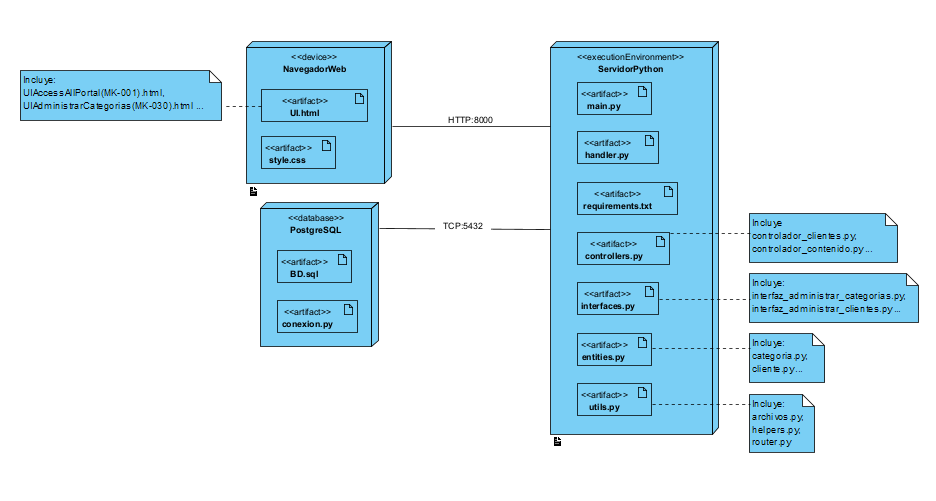
\includegraphics[width=0.95\linewidth]{Media/4_Disenio/despliegue.png}
    \caption{Diagrama de despliegue del sistema \textbf{QuickContentMedia}}
    \label{DiagDesp}
\end{figure}

\textbf{Archivo:} Diagrama de despliegue (formato Visual Paradigm) \\
\textbf{Link de descarga:} \linkDiagramaDespliegue \\

\textbf{Pasos de ejecución:}
\begin{itemize}
    \item Ingresar al repositorio en GitHub usando el link proporcionado y descargar el archivo \texttt{QCM\_despliegue.vpp}.
    \item En la pestaña Deployment diagram abrir DiagramaDespliegueQCM.
\end{itemize}

\subsubsection{Diccionario de despliegue}

\begin{table}[H]
\centering
\caption{Diccionario de Nodos de Despliegue}
\label{tab:diccionario_nodos_despliegue}
\begin{tabular}{|p{1cm}|p{2cm}|p{3.5cm}|p{3cm}|p{3cm}|p{3cm}|}
\hline
\textbf{ID} & \textbf{Nodo} & \textbf{Descripción} & \textbf{Artefactos} & \textbf{Descripción Artefactos} & \textbf{Comunicación} \\ \hline

NO-01 & Navegador Web & Navegador utilizado por el usuario para acceder a la aplicación. Compatible con Chrome, Firefox, Edge, Safari y Opera. & 
\begin{itemize}[leftmargin=*, noitemsep]
    \item UI.html
    \item style.css
\end{itemize} & 
HTML para la interfaz de usuario y CSS para estilos visuales. & 
HTTP:8000 hacia NO-02 Servidor Python \\ \hline

NO-02 & Servidor Python & Ambiente de ejecución de la lógica del backend implementada en Python 3.12, con framework Flask. & 
\begin{itemize}[leftmargin=*, noitemsep]
    \item main.py
    \item handler.py
    \item requirements.txt
    \item controllers.py
    \item interfaces.py
    \item entities.py
    \item utils.py
\end{itemize} & 
Scripts en Python que implementan la lógica de negocio, manejo de rutas, controladores y entidades. & 
HTTP:8000 desde NO-01 \newline TCP:5432 hacia NO-03 \\ \hline

NO-03 & PostgreSQL & Motor de base de datos relacional usado para persistencia de datos. Se utiliza la versión 17 de PostgreSQL. & 
\begin{itemize}[leftmargin=*, noitemsep]
    \item BD.sql
    \item conexion.py
\end{itemize} & 
Script de definición de la base de datos y conexión mediante Python a PostgreSQL. & 
TCP:5432 desde NO-02 Servidor Python \\ \hline

\end{tabular}
\end{table}

